\documentclass[11pt]{article}

\usepackage{fullpage,times}%charter}
\usepackage{color}
\usepackage{float}
\usepackage{tikz}
\usetikzlibrary{arrows.meta}

%% macros
\newcommand{\ax}[1]{\texttt{AX}(#1)}
\newcommand{\ex}[1]{\texttt{EX}(#1)}
\newcommand{\af}[1]{\texttt{AF}(#1)}
\newcommand{\ef}[1]{\texttt{EF}(#1)}
\newcommand{\ag}[1]{\texttt{AG}(#1)}
\newcommand{\eg}[1]{\texttt{EG}(#1)}
\newcommand{\au}[2]{\texttt{A}(#1\ \texttt{U}\ #2)}
\newcommand{\eu}[2]{\texttt{E}(#1\ \texttt{U}\ #2)}
\newcommand{\sem}[1]{[\!\![#1]\!\!]}

\newcommand{\sol}[1]{{\color{blue}#1}}

\begin{document}

\hrule
\smallskip

\noindent
You can review the latex source for this assignment-file to
learn and use latex to prepare your homework submission. You will see
the use of macros (to write uniformly formatted text), different
text-styles (emphasized, bold-font), different environments (figures,
enumerations).

It is not required that you use exactly this latex source to prepare
your submission. 
\smallskip
\hrule


\begin{center}
{\Large\bf Homework 1 (CTL): ComS/CprE/SE 412, ComS 512}

\medskip

Due-date: Feb 7 at 11:59PM.

\medskip


\end{center}

\noindent
\textbf{
Submit online on Canvas two files: the source file in latex format and
the pdf file generated from latex. Name your files:
$\langle\mbox{your-net-id}\rangle$-hw1.$\langle\mbox{tex/pdf}\rangle$.
}

\hrule
\noindent
\smallskip

\emph{ Homework must be individual's original work. Collaborations and
  discussions of any form with any students or other faculty members
  or soliciting solutions on online forums are not allowed. Please
  review the academic dishonesty policy on our syllabus. If you have
  any questions/doubts/concerns, post your questions/doubts/concerns
  on Piazza and ask TA/Instructor.}

\smallskip
\hrule

\begin{enumerate}

\item
Consider the following Kripke structure, with $p\in L(s_0) \cap L(s_2)$ and
$q\in L(s_2)$.
\begin{center}
    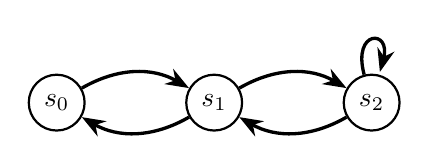
\begin{tikzpicture}
\begin{scope}[every node/.style={circle,thick,draw}]
    \node (s0) at (0,0) {$s_0$};
    \node (s1) at (2,0) {$s_1$};
    \node (s2) at (4,0) {$s_2$};
\end{scope}

\begin{scope}[>={Stealth[black]},
              every node/.style={fill=white,circle},
              every edge/.style={draw=black,very thick}]
    \path [->] (s0) edge[bend left=30] (s1);
    \path [->] (s1) edge[bend left=30] (s0);
    \path [->] (s1) edge[bend left=30] (s2);
    \path [->] (s2) edge[bend left=30] (s1);
    \path [->] (s2) edge[loop above] (s2);
\end{scope}
\end{tikzpicture}
\end{center}
Identify the set of states that satisfy each of the following:
\begin{enumerate}
\item $\ex{q}$

  
\item $\ax{p}$
  
\item $\ax{q}$

\item $\ag{p}$
  
\item $\eg{p}$

\item $\af{p}$

\item $\ag{\ex{p}}$
  
\item $\ag{\af{p}}$
  
\end{enumerate}
\hfill(16 pts)


\textbf{Answer}: The tree of computation is - 

\begin{enumerate}
\item $ \{s_1, s_2\} $ 

  
\item $ \{s_1\}$
  
\item $\{ \}$

\item $\{ \}$
  
\item $\{ s_2\}$

\item $\{ s_0, s_1, s_2\}$

\item $\{\}$
  
\item $\{s_0, s_1, s_2\}$
  
\end{enumerate}

\item Express the following statements as CTL formula:\hfill (4+4+6 pts)
\begin{enumerate}

\item
Along all paths \textbf{withdraw-money} is never true after
\textbf{invalid-login}.

\textbf{Answer}: AG (\textbf{invalid-login} $\Rightarrow$ AXAG  \textbf{withdraw-money})

\item
Along all execution sequences of an elevator behavior, if the elevator
door is \textbf{open} then the door remains \textbf{open} until a
\textbf{request-to-move} is sent to the elevator.

\textbf{Answer}: AG ((\textbf{open} $\Rightarrow$ AG  \textbf{open}) U \textbf{request-to-move})

\item 
Whenever proposition \textbf{request-site-update} is true in a state,
it is followed in zero or more steps by a state where proposition
\textbf{updating-site} is true, which in turn is followed in one or
more steps by a state where \textbf{update-complete} is true.

\textbf{Answer}: AG (( \textbf{request-site-update} $\Rightarrow $AF \textbf{updating-site} ) $\Rightarrow$ AXAF \textbf{update-complete})


\end{enumerate}


\item To disprove that two CTL formula are equivalent, you are
  required to draw a Kripke structure and identify a state in that
  structure, which satisfies one of the formula and does not satisfy
  the other. For instance, in order to disprove that
  $\ex{p}\ \land\ \ex{q}$ and $\ex{p\ \land\ q}$ are equivalent, we can
  draw the following the Kripke structure:

  \begin{center}
  \begin{tabular}{cc}
  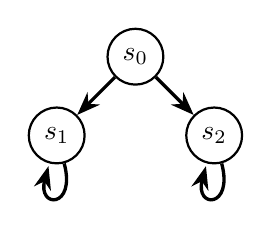
\begin{tikzpicture}
\begin{scope}[every node/.style={circle,thick,draw}]
    \node (s0) at (0,0) {$s_0$};
    \node (s1) at (-1,-1) {$s_1$};
    \node (s2) at (1,-1) {$s_2$};
\end{scope}

\begin{scope}[>={Stealth[black]},
              every node/.style={fill=white,circle},
              every edge/.style={draw=black,very thick}]
    \path [->] (s0) edge (s1);
    \path [->] (s0) edge  (s2);
    \path [->] (s1) edge[loop below] (s1);
    \path [->] (s2) edge[loop below] (s2);
\end{scope}
  \end{tikzpicture}
  &
  %%
  \begin{tabular}{l}
    $L(s_1) = \{p\}$, $L(s_2) = \{q\}$
    \end{tabular}
  \end{tabular}
\end{center}
We present the labels for the relevant states in the Kripke structure
and state that $s_0$ satisfies $\ex{p}\ \land\ \ex{q}$ and $s_0$ does
not satisfy $\ex{p \land q}$. This is because there exists a path from
$s_0$ where in the very next state $s_1$ the proposition $p$ is true;
thus conforming that $s_0$ satisfies $\ex{p}$ (similarly, one can justify
the satisfiability of $\ex{q}$ at state $s_0$). On the other hand,
there exists no path from $s_0$, where in the very next state both $p$
and $q$ are satisfied. 
\smallskip

  
Disprove that the two CTL formula $\af{p \land q}$ and
$\af{p} \land \af{q}$ are equivalent.  \hfill (5 pts)

\textbf{Answer}:

$\af{p \land q}$ implies that $p \land q$ is true sometimes in all possible future states from starting state.  However, $\af{p} \land \af{q}$ says that "In all possible future states, p must be true, and in all possible future states, q must be true".  Therefore, p and q does not necessarily true in one state to satisfy $\af{p} \land \af{q}$, but $\af{p \land q}$ demands p and q to be  true in the same state. 



  \begin{center}
  \begin{tabular}{cc}
  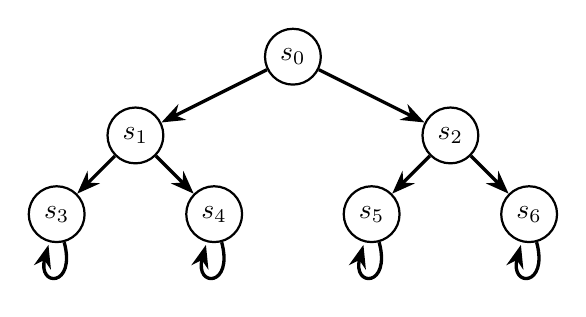
\begin{tikzpicture}
\begin{scope}[every node/.style={circle,thick,draw}]
    \node (s0) at (0,0) {$s_0$};
    \node (s1) at (-2,-1) {$s_1$};
    \node (s2) at (2,-1) {$s_2$};
    
    \node (s3) at (-3,-2) {$s_3$};
    \node (s4) at (-1,-2) {$s_4$};

    \node (s5) at (1,-2) {$s_5$};
    \node (s6) at (3,-2) {$s_6$};
\end{scope}

\begin{scope}[>={Stealth[black]},
              every node/.style={fill=white,circle},
              every edge/.style={draw=black,very thick}]
    \path [->] (s0) edge (s1);
    \path [->] (s0) edge  (s2);
    \path [->] (s1) edge (s3);
    \path [->] (s1) edge (s4);
    \path [->] (s3) edge[loop below] (s3);
    \path [->] (s4) edge[loop below] (s4);


    \path [->] (s2) edge (s5);
    \path [->] (s2) edge (s6);
    \path [->] (s5) edge[loop below] (s5);
    \path [->] (s6) edge[loop below] (s6);
    
\end{scope}
  \end{tikzpicture}
  &
  %%
  \begin{tabular}{l}
    $L(s_1) = \{p\}$, $L(s_3) = \{q\}$, $L(s_4) = \{q\}$ \\ $L(s_2) = \{q\}$, $L(s_5) = \{p\}$, $L(s_6) = \{p\}$
    \end{tabular}
  \end{tabular}
\end{center}

The above Kripke structure satisfies $\af{p} \land \af{q}$, but it does not satisfy $\af{p \land q}$. Therefore, it can be said that these two properties are not equivalent. 


% \begin{figure}[H]
%     \centering
%     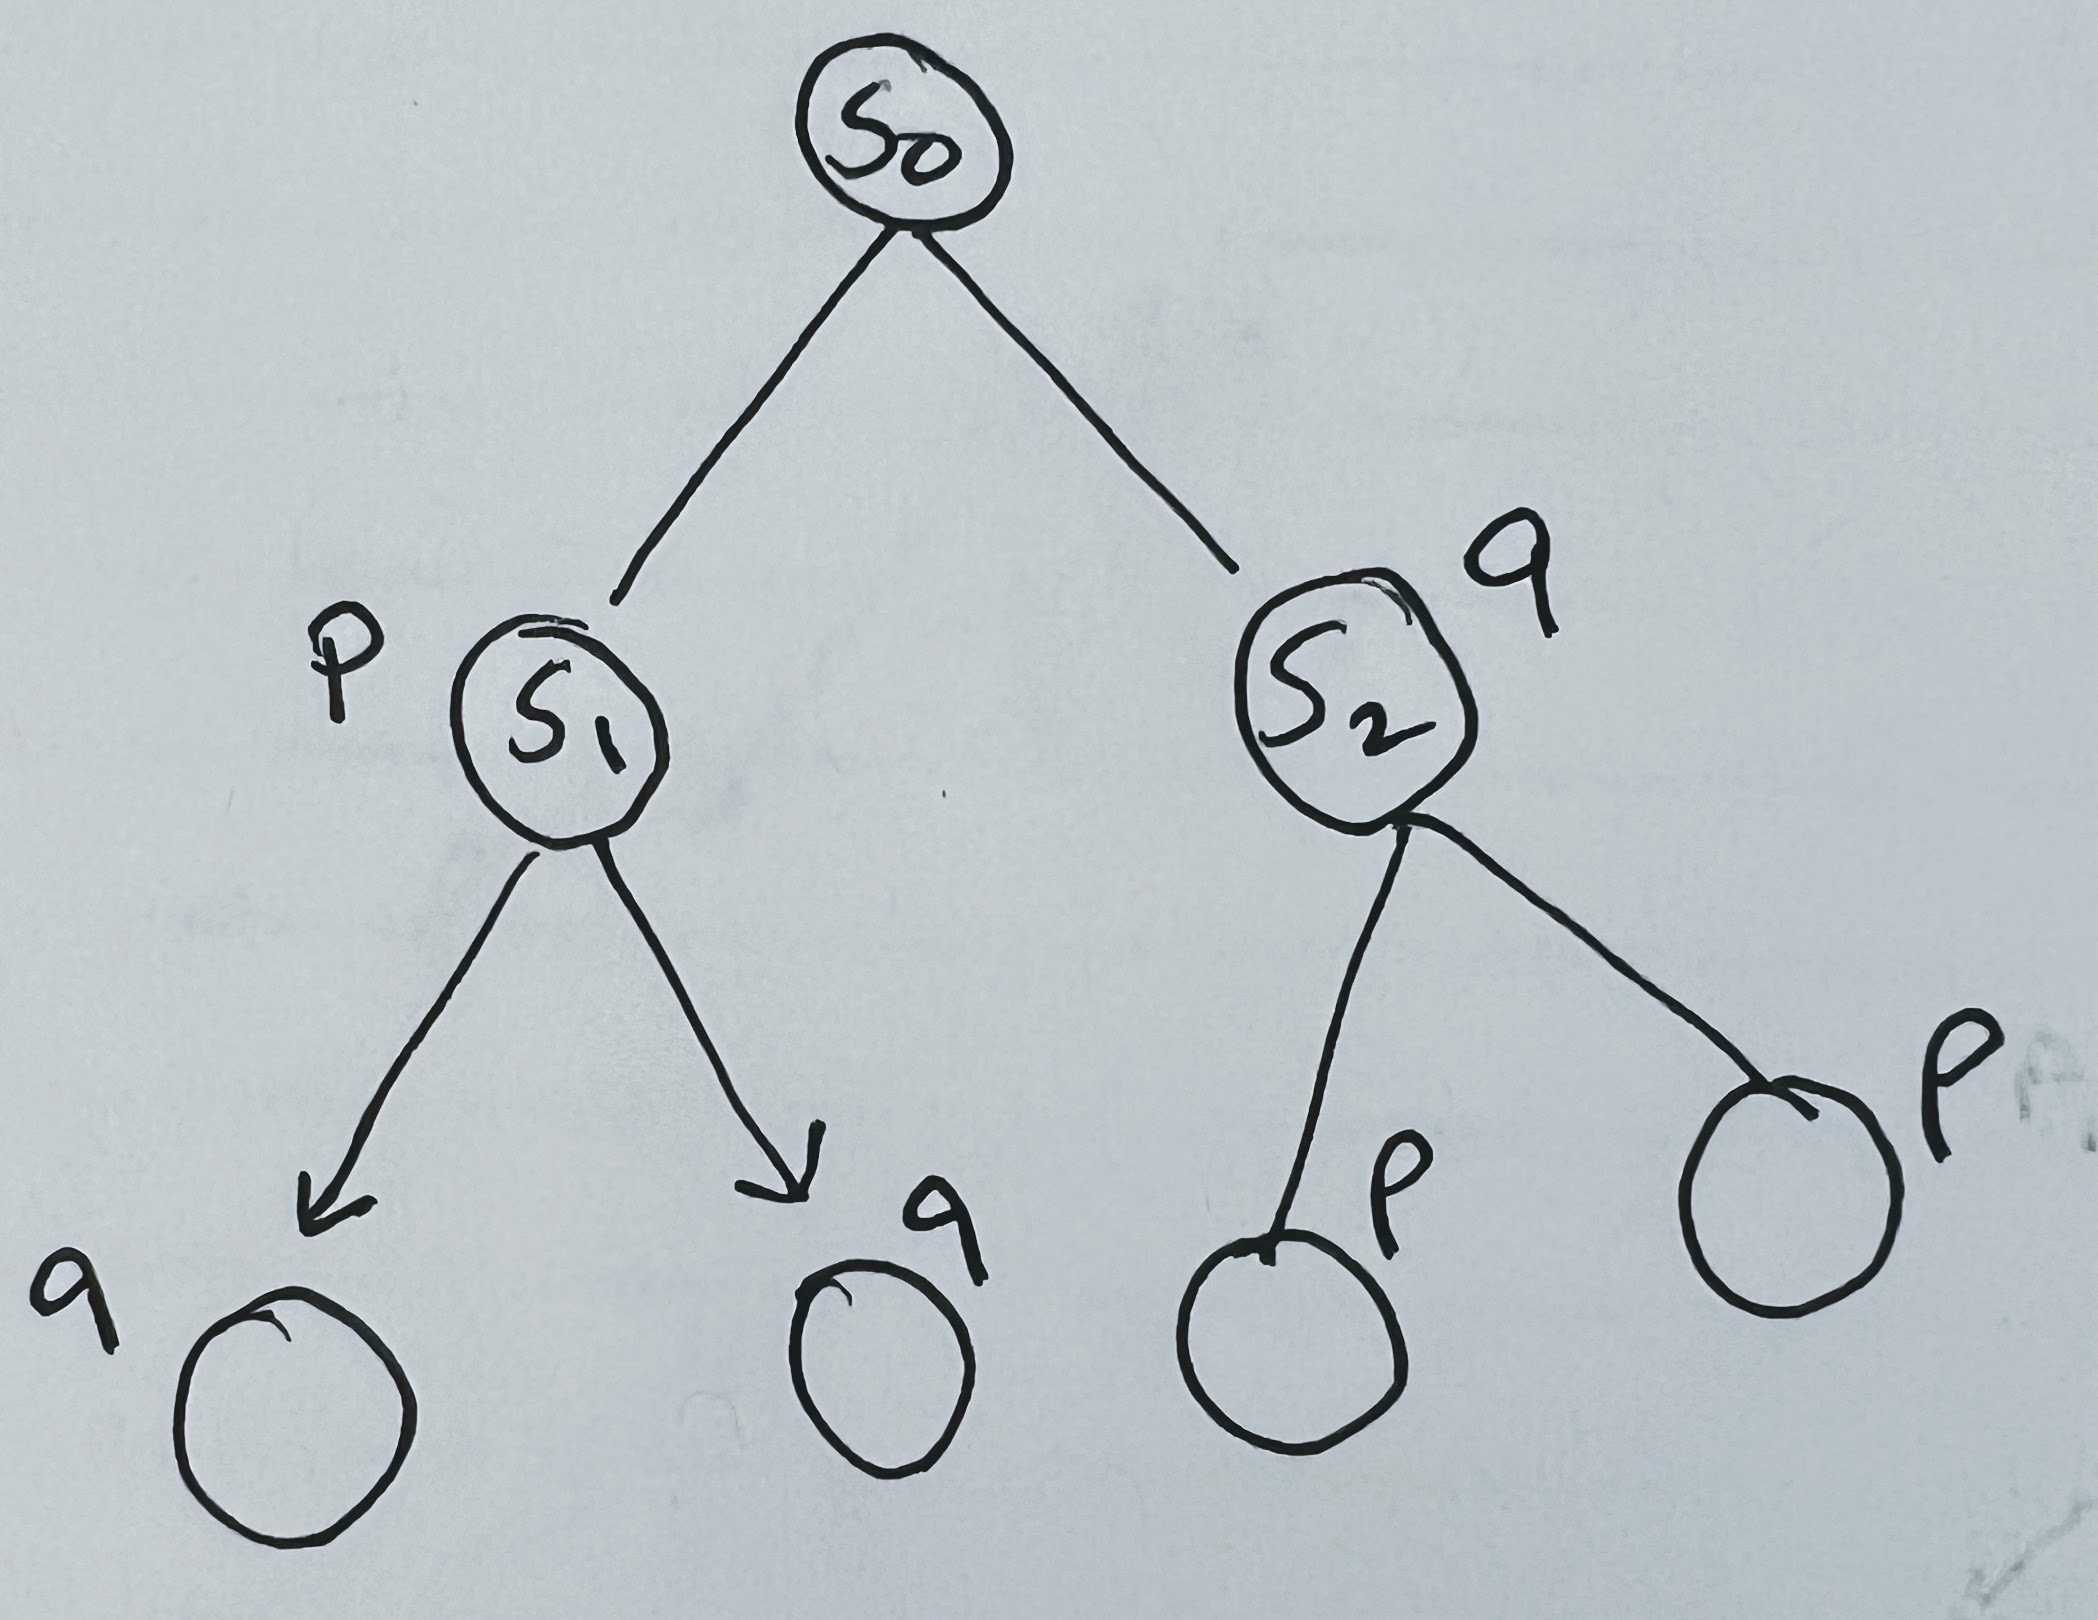
\includegraphics[width=7cm]{images/1_3.jpg}
%     \caption{ The Kripke structure dissatisfying $\af{p \land q}$ and
% $\af{p} \land \af{q}$ }
%     \label{kripke_struc}
% \end{figure}



\item
To prove that one formula (say, $\varphi_1$) is ``stronger'' than
another (say, $\varphi_2$), you need to prove that whenever in any
state in any Kripke structure $\varphi_1$ holds, $\varphi_2$ holds in
that state as well. In other words, $\varphi_1$ is ``stronger'' than
$\varphi_2$ if and only if $\varphi_1\Rightarrow\varphi_2$ is a
tautology (always evaluates to true). For instance, to prove that
$\ax{p}$ is stronger than $\ex{p}$ we can write:
%% math environment starts
\[
\begin{array}{rcl}
  \forall s. s\in \sem{\ax{p}} & \Leftrightarrow & \forall \pi\in Path(s): \pi[1] \in \sem{p} \\
                               & \Rightarrow &     \exists \pi\in Path(s): \pi[1] \in \sem{p} \\
                               & \Rightarrow & s \in \sem{\ex{p}}
\end{array}
\]
%% math environment ends
%%
To disprove that $\ex{p}$ is stronger that $\ax{p}$, you will draw a
Kripke structure and present a state in the Kripke structure that
satisfies $\ex{p}$ but does not satisfy $\ax{p}$ (see the Kripke
structure example in the previous problem).

Prove or disprove $\ag{p\ \land\ q}$ is stronger than $\ag{p\ \Rightarrow\ \af{q}}$.

\textbf{Answer}:

Let's simplify $\ag{p \Rightarrow \af{q}}$. 
\[
\begin{array}{rcl}
  \forall s. s\in \sem{\ag{p\ \Rightarrow\ \af{q}}} & \Leftrightarrow & \forall \pi\in Path(s): \pi[0] \in \sem{p\ \Rightarrow\ \af{q}} \\
                               & \Rightarrow &     \forall \pi\in Path(s): \pi[0] \in \sem{ \neg p \lor \af{q}} \\
                               & \Rightarrow &     \forall \pi\in Path(s): \pi[0] \in \sem{ \af{q}} \\
                               & \Rightarrow &     \forall \pi\in Path(s): \pi[0] \in \sem{ {q}} \\
\end{array}
\]

When $\ag{p \Rightarrow \af{q}}$ holds in $s$, it is immediately true that $p \Rightarrow \af{q}$ holds for all successors of s, including $s$ itself. We can rewrite $p \Rightarrow \af{q}$ as $\neg p \lor \af{q}$, which implies either $\neg p$ or $\af{q}$ true in s and its successors. without loss of generality, we can write q holds in state $s$. 

$\ag{p \land q}$ implies $p \land q$ holds in all successors of $s$ including $s$ itself. As both $p$ and $q$ holds in state $s$, which suffices to show that $p\ \Rightarrow\ \af{q}$ immediately true at that state. The Kripke structure satisfying $\ag{p \land q}$ is provided below. 


  \begin{center}
  \begin{tabular}{cc}
  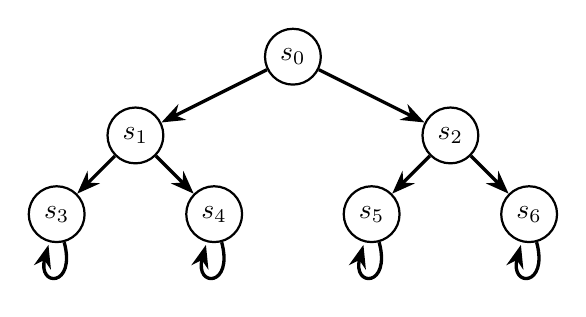
\begin{tikzpicture}
\begin{scope}[every node/.style={circle,thick,draw}]
    \node (s0) at (0,0) {$s_0$};
    \node (s1) at (-2,-1) {$s_1$};
    \node (s2) at (2,-1) {$s_2$};
    
    \node (s3) at (-3,-2) {$s_3$};
    \node (s4) at (-1,-2) {$s_4$};

    \node (s5) at (1,-2) {$s_5$};
    \node (s6) at (3,-2) {$s_6$};
\end{scope}

\begin{scope}[>={Stealth[black]},
              every node/.style={fill=white,circle},
              every edge/.style={draw=black,very thick}]
    \path [->] (s0) edge (s1);
    \path [->] (s0) edge  (s2);
    \path [->] (s1) edge (s3);
    \path [->] (s1) edge (s4);
    \path [->] (s3) edge[loop below] (s3);
    \path [->] (s4) edge[loop below] (s4);


    \path [->] (s2) edge (s5);
    \path [->] (s2) edge (s6);
    \path [->] (s5) edge[loop below] (s5);
    \path [->] (s6) edge[loop below] (s6);
    
\end{scope}
  \end{tikzpicture}
  &
  %%
  \begin{tabular}{l}
    $L(s_1) = \{p, q\}$, $L(s_3) = \{p, q\}$, $L(s_4) = \{p, q\}$ \\ $L(s_2) = \{p, q\}$, $L(s_5) = \{p, q\}$, $L(s_6) = \{p, q\}$
    \end{tabular}
  \end{tabular}
\end{center}

So, we can say that the formula $\ag{p \land q}$ is stronger than $\ag{p \Rightarrow \af{q}}$.

\hfill (5 pts)

\item \textbf{Extra Credit for 412; Required problem for 512.}
  We will define a new operator $A\circ$
  as follows. A state $s$ satisfies $\texttt{A}(\varphi_1\ \circ\ \varphi_2)$
  if and only if for all paths starting from $s$ at least one of the
  following holds
\begin{itemize}
\item there exists a state where $\varphi_2$ is
  satisfied and before that $\varphi_1$ holds in all states in the
  path
\item all states in the path satisfy $\varphi_1$ and not
  $\varphi_2$
\end{itemize}
Prove or disprove that 
\begin{enumerate}
\item $A(p\ \circ\ \mbox{false})$ can be expressed
  in CTL.
  
\textbf{Answer:} Let's first consider the first condition, which says for all paths starting from $s$ finally satisfies $false$, and before that $p$ holds in all state. In CTL, there is no way to satisfy $false$ formula along all paths. So, $A(p\ \circ\ \mbox{false})$ does not hold the first formula. 

The second condition says for all paths starting from $s$ satisfy $p \land \neg false \Rightarrow p \land true \Rightarrow p $. Which can be written as $\ag{p}$. 

Therefore, $A(p\ \circ\ \mbox{false})$ can be expressed using CTL formula $\ag{p}$. 


\item $A(\mbox{false}\ \circ\ p)$ can be expressed in CTL.

\textbf{Answer:}

Let's first try to express the first condition in CTL, first condition says that for all paths there exists a state where $p$ is
  satisfied, and before that $false$ holds in all states in the path. It can be immediately inferred that we cannot express this in CTL because these paths have negative path quantification, which cannot be expressed in CTL. 


  The second condition says that  $\ag{false \land \neg p} \Rightarrow \ag{false}$. Which is also not supported by CTL. 

  Therefore, $A(\mbox{false}\ \circ\ p)$ cannot be expressed in CTL. 

\end{enumerate}
\hfill(10pts)

\textbf{Answer}: 

The first condition "there exists a state where $\varphi_2$ is satisfied and before that $\varphi_1$ holds in all states in the
  path" and the second condition, "all states in the path satisfy $\varphi_1$ and not
  $\varphi_2$" can be represented as $\ag{\varphi_1 \rightarrow \af{\varphi2}} $ and $ \ag{\varphi_1 \land \neg \varphi_2}$ respectively.

  \begin{enumerate}
\item $A(p\ \circ\ \mbox{false})$ can be written as follows-

$$\ag{p \rightarrow \af{false}} \lor \ag{p \land \neg false}$$

$$\Rightarrow \ag{\neg p \lor \af{false}} \lor \ag{p \land true}$$

$$\Rightarrow  \ag{p}$$




\item $A(\mbox{false}\ \circ\ p)$ cannot be expressed in CTL. If we write this formula like the above,

$$\ag{false \rightarrow \af{p}} \lor \ag{false \land \neg p}$$
$$\rightarrow $$

\end{enumerate}

% The formula $\texttt{A}(\varphi_1\ \circ\ \varphi_2)$ can be defined using existing CTL formulas as follows:

% $\texttt{A}(\varphi_1\ \circ\ \varphi_2) \equiv \texttt{AG}(\varphi_1 \rightarrow \texttt{EF}(\varphi_2)) \land \texttt{AG}(\neg \varphi_2 \rightarrow \texttt{AX}(\varphi_1))$

% Explanation:

% $\texttt{AG}(\varphi_1 \rightarrow \texttt{EF}(\varphi_2))$ says that if $\varphi_1$ is satisfied, then there exists a state where $\varphi_2$ is satisfied.

% $\texttt{AG}(\neg \varphi_2 \rightarrow \texttt{AX}(\varphi_1))$ says that if $\varphi_2$ is not satisfied, then $\varphi_1$ holds in all states in the path.

% Together, these two formulas capture the condition that for all paths starting from $s$, either $\varphi_2$ is satisfied and $\varphi_1$ holds in all states in the path before that, or $\varphi_1$ holds in all states in the path and $\varphi_2$ is not satisfied.


% \textbf{Answer}: $A(p\ \circ\ \mbox{false})$ can be expressed in CTL: True. This operator can be expressed using the CTL formula $\ag{p} \vee \ax{\neg p \land \neg q}$. Here, $\ag{p}$ means "in all possible futures, $p$ holds". $\ax{\neg p \land \neg q}$ means "for all next states, both $p$ and $q$ do not hold". These two formulas capture the two conditions specified in the definition of the operator $\texttt{A}(\varphi_1\ \circ\ \varphi_2)$.

% $A(\mbox{false}\ \circ\ p)$ can be expressed in CTL: False. This operator cannot be expressed using standard CTL, because it requires a negative path quantification, which is not supported by standard CTL. In standard CTL, all paths are considered, positive or negative.

\end{enumerate}



\end{document}

